\documentclass[
	12pt, 
	a4paper, 
	oneside,
	parskip=half*, % Line spacing for paragraphs
	openany,  % openany -> on which page should new chapters start
	listof=totoc, % Include listings in the table of contents
	bibliography=totoc, % adding a bibliography to the table of contents
	index=totoc, % add index directory to the table of contents
  toc=chapterentrywithdots, % Set dots in the table of contents also for chapters
  numbers=noenddot, % removes the last dot after X.X.X.
  %chapterprefix=true % changes the display of the chapter, adds "Chapter" to the chapter number
]{scrbook}


\usepackage[utf8]{inputenc}
\usepackage[english]{babel}
\usepackage{url}
\usepackage[autostyle=true,german=quotes]{csquotes}
\usepackage[T1]{fontenc}
\usepackage{pdfpages}
\usepackage{textcomp}
\usepackage{amsmath} % math environment
\usepackage{scrhack}
\usepackage{multirow}
\usepackage{diagbox}
\usepackage{makecell}
\usepackage{rotating}
\usepackage{tikz}
\usepackage{array}
\usepackage{float}
\usepackage{tabularx}
\usepackage{newtxtext}
\usepackage{booktabs}
\usepackage{longtable}
\usepackage{enumitem}
\usepackage[titles]{tocloft}
\usepackage[a4paper, margin=2.5cm]{geometry}
\usepackage{titletoc}


% ---------------------------
% |    Meta-Data for PDF    |
% ---------------------------
\usepackage[
  pdftex,
  pdfauthor={Hauke Schwarz},
  pdftitle={Thesis},
  pdfsubject={Master Thesis},
  pdfkeywords={Thesis;Template;LaTeX},
  pdfproducer={LaTeX},
  pdfcreator={pdfLaTeX},
  pdfduplex={DuplexFlipLongEdge}, %Alt.: Simplex or DuplexFlipShortEdge 
  pdflang={en},
  bookmarksopen,
  bookmarksnumbered
]{hyperref}


% ------------------
% |    Settings    |
% ------------------
\usepackage[
    backend=biber, 
    style=authoryear-icomp, % alphabetic
    citestyle=authoryear-icomp, % alphabetic, authortitle
    date=short,
    % backref=true, % Display pages on which the reference is used
    maxnames=2, % affects the cites
    maxbibnames=3, % affects the bibliography
    pagetracker=true,
    isbn=false,    
    % block=ragged, % break urls
    % firstinits=true, % shorten first names
    backrefstyle=three+ % Combine pages
]{biblatex}

% Distance between bibliographical references
\setlength{\bibitemsep}{.5em}

% Indentation after the first line
\setlength{\bibhang}{2em}

% URL in the bibliography is in angle brackets
\DeclareFieldFormat{url}{<\url{#1}>}

% break too long urls
\setcounter{biburllcpenalty}{7000}
\setcounter{biburlucpenalty}{8000}

% Source of the bibliography file
\addbibresource{literature/thesis_lib.bib}

% add comma 
\renewcommand*{\nameyeardelim}{\addcomma\space}



% graphics
\usepackage{graphicx}
\graphicspath{ {images/} }
\DeclareGraphicsExtensions{.pdf,.png,.jpg,.jpeg,.gif}

% captions
\usepackage{caption}
\usepackage{subcaption}
% Table layout
\setlength{\tabcolsep}{0.5em} % for the horizontal padding
{\renewcommand{\arraystretch}{1.2} % for the vertical padding

% Table captions
\usepackage{caption} 
\captionsetup[table]{belowskip=12pt,aboveskip=4pt}
\usepackage{diagbox}

% Rotate tables
\usepackage{rotating}
\usepackage{varwidth}

% Footnotes with tables
\usepackage{footnote}
\makesavenoteenv{figure}

% Line breaks in table cells
\newcommand{\specialcell}[2][c]{%
  \begin{tabular}[#1]{@{}c@{}}#2\end{tabular}
}

% rotate content of table cell
\def\rot{\rotatebox} % usage: \rot{angle}{content}
% You can visit this website to find more color codes for LaTeX
% http://latexcolor.com/s

\usepackage{xcolor}

% colors
\definecolor{white}{rgb}{1,1,1}
\definecolor{black}{rgb}{0,0,0}
\definecolor{middlegray}{rgb}{0.5,0.5,0.5}
\definecolor{lightgray}{rgb}{.95,.95,.95}
\definecolor{arsenic}{rgb}{0.23, 0.27, 0.29}
\definecolor{arsenicLight}{rgb}{0.20, 0.20, 0.20}
\definecolor{darkgray}{rgb}{.4,.4,.4}
\definecolor{purple}{rgb}{0.65, 0.12, 0.82}
\definecolor{orange}{rgb}{0.8,0.3,0.3}
\definecolor{yac}{rgb}{0.6,0.6,0.1}
\definecolor{green}{rgb}{.2,0.6,0.3}
\definecolor{azure}{rgb}{0.0, 0.5, 1.0}
\definecolor{editorGray}{rgb}{0.95, 0.95, 0.95}
\definecolor{editorOcher}{rgb}{1, 0.5, 0}
\definecolor{editorGreen}{rgb}{0, 0.5, 0}
\definecolor{orange}{rgb}{1,0.45,0.13}		
\definecolor{olive}{rgb}{0.17,0.59,0.20}
\definecolor{brown}{rgb}{0.69,0.31,0.31}
\definecolor{purple}{rgb}{0.38,0.18,0.81}
\definecolor{lightblue}{rgb}{0.1,0.57,0.7}
\definecolor{lightred}{rgb}{1,0.4,0.5}

\definecolor{vscodered}{HTML}{E53935}
\definecolor{vscodelightred}{HTML}{EF5350}
\definecolor{vscodeblue}{HTML}{1565C0}
\definecolor{vscodegreen}{HTML}{66BB6A}

\definecolor{lightblack}{HTML}{212121}
\definecolor{darkraspberry}{rgb}{0.53, 0.15, 0.34}

% blue hues
\definecolor{bleudefrance}{rgb}{0.19, 0.55, 0.91}
\definecolor{brandeisblue}{rgb}{0.0, 0.44, 1.0}
\definecolor{blue(ncs)}{rgb}{0.0, 0.53, 0.74}
\definecolor{coolblack}{rgb}{0.0, 0.18, 0.39}

% red hues
\definecolor{coralred}{rgb}{1.0, 0.25, 0.25}
\definecolor{darkred}{rgb}{0.55, 0.0, 0.0}

% geometry
\usepackage{geometry}
\geometry{left=25mm, right=25mm, top=25mm, bottom=30mm}

\usepackage[automark]{scrlayer-scrpage}
\pagestyle{scrheadings}
\automark*[section]{}
\clearpairofpagestyles
\ohead{\headmark} % name of the current section
\ihead{}
\ofoot{\thepage} % page number

% Define a new page style for the first page of each chapter
\deftripstyle{chapterfirst}{}{}{}{}{}{\pagemark}
\renewcommand*{\chapterpagestyle}{chapterfirst}




% footnote gap
%\addtolength{\skip\footins}{1ex}
%\addtolength{\footnotesep}{0.5ex}

% prevent footnote page break
\interfootnotelinepenalty=10000

% line spacing
\usepackage[onehalfspacing]{setspace}

% text does not have to go to the end of a page
\raggedbottom

% space before and after chapter headings
\RedeclareSectionCommand[beforeskip=0pt,afterskip=.6cm,font=\fontsize{18}{20}\selectfont]{chapter}
%\RedeclareSectionCommand[beforeskip=10pt,afterskip=.3cm,font=\fontsize{18}{25}\selectfont]{section}
%\RedeclareSectionCommand[beforeskip=10pt,afterskip=.3cm,font=\fontsize{16}{25}\selectfont]{subsection}
%\RedeclareSectionCommand[beforeskip=0pt,afterskip=.3cm,font=\fontsize{14}{25}\selectfont]{subsubsection}

\usepackage{mwe}

% chapter style
\renewcommand*{\chapterformat}{%
  \thechapter\enskip
  \textcolor{gray!70}{\rule[-\dp\strutbox]{1pt}{\baselineskip}}\enskip
}
\setkomafont{disposition}{\normalcolor\bfseries}

% adjust paragraphs
%\addtokomafont{paragraph}{\itshape}
%\setkomafont{subsubsection}{\large}
%\setkomafont{paragraph}{\normalsize\itshape}
\setkomafont{paragraph}{\normalsize}

% layout of the paragraphs
% paragraphs look like the subsubsections
\RedeclareSectionCommands[
    beforeskip=-3.25ex plus -1ex minus -0.2ex,
    afterskip=1sp, % smallest possible positive value
]{paragraph,subparagraph}

% Bold caption labels
\setkomafont{captionlabel}{\normalsize\bfseries} 
% \usepackage[font=sf]{caption} % Captions without serifs
\usepackage{listings}
\usepackage[many]{tcolorbox}

% name of listings in the toc
\renewcommand\lstlistlistingname{Listingverzeichnis}

% general settings for listing
\lstset{
    xleftmargin=1.1cm,
    belowskip=2em,
    basicstyle=\fontsize{10}{15}\ttfamily,
    basewidth  = {.5em,0.4em},
    captionpos=t,
    lineskip={2pt},
    backgroundcolor=\color{white},
    framextopmargin=6pt,
    framexrightmargin=0pt,
    framexleftmargin=0.9em,    
    framexbottommargin=6pt, 
    frame=l,
%    frame=single,        
%    frame=tb, framerule=0pt,    
    framesep=6.5mm,
    fillcolor=\color{white},
    rulecolor=\color{middlegray},
    numbers=left,
    numberstyle=\normalfont\color{middlegray},
%    numberstyle=\footnotesize,    
    numbersep=10pt,
    abovecaptionskip=10pt, %space above the caption
    belowcaptionskip=10pt, %space below the caption
    extendedchars=true,
    showstringspaces=false,
    showspaces=false,
    stepnumber=1, % the step between two line-numbers. If it is 1 each line will be numbered
    tabsize=2,
    breaklines=true,
    showtabs=false,
    upquote=true,
    % German umlauts
    literate=%
    {Ö}{{\"O}}1
    {Ä}{{\"A}}1
    {Ü}{{\"U}}1
    {ß}{{\ss}}1
    {ü}{{\"u}}1
    {ä}{{\"a}}1
    {ö}{{\"o}}1
}

% define language
\lstdefinelanguage{JavaScript}{
    keywords={typeof, new, true, false, catch, then, function, return, null, catch, switch, var, if, in, while, do, else, case, break, default},
    keywordstyle=\color{editorGreen}\bfseries,
    ndkeywords={class, export, boolean, throw, implements, import, this, const},
    ndkeywordstyle=\color{vscodeblue}\bfseries,
    identifierstyle=\color{black},
    sensitive=false,
    comment=[l]{//},
    morecomment=[s]{/*}{*/},
    commentstyle=\color{editorGreen}\ttfamily,
    stringstyle=\color{darkred}\ttfamily,
    morestring=[b]',
    morestring=[b]"
}

\lstdefinelanguage{SQL}{
    keywords={select, where, from},
    keywordstyle=\color{editorGreen}\bfseries,
    ndkeywords={},
    ndkeywordstyle=\color{vscodeblue}\bfseries,
    identifierstyle=\color{black},
    sensitive=false,
    comment=[l]{--},
    morecomment=[s]{/*}{*/},
    commentstyle=\color{editorGreen}\ttfamily,
    stringstyle=\color{darkred}\ttfamily,
    morestring=[b]',
    morestring=[b]"
}


\lstdefinelanguage{HTML5}{
  language=html,
  sensitive=true,	
  alsoletter={<>=-},	
  morecomment=[s]{<!-}{-->},
  tag=[s],
  otherkeywords={
  % General
  >,
  % Standard tags
	<!DOCTYPE,
  </html, <html, <head, <title, </title, <style, </style, <link, </head, <meta, />,
	% body
	</body, <body,
	% Divs
	</div, <div, </div>, 
	% Paragraphs
	</p, <p, </p>,
	% scripts
	</script, <script,
  % More tags...
  <canvas, /canvas>, <svg, <rect, <animateTransform, </rect>, </svg>, <video, <source, <iframe, </iframe>, </video>, <image, </image>, <header, </header, <article, </article
  },
  ndkeywords={
  % General
  =,
  % HTML attributes
  charset=, src=, id=, width=, height=, style=, type=, rel=, href=,
  % SVG attributes
  fill=, attributeName=, begin=, dur=, from=, to=, poster=, controls=, x=, y=, repeatCount=, xlink:href=,
  % properties
  margin:, padding:, background-image:, border:, top:, left:, position:, width:, height:, margin-top:, margin-bottom:, font-size:, line-height:,
	% CSS3 properties
  transform:, -moz-transform:, -webkit-transform:,
  animation:, -webkit-animation:,
  transition:,  transition-duration:, transition-property:, transition-timing-function:,
  }
}

\lstdefinestyle{html} {%
  % Code design
  keywordstyle=\color{lightblack}\bfseries,
  ndkeywordstyle=\color{lightblack}\bfseries,
  identifierstyle=\color{lightblack},
  commentstyle=\color{green}\ttfamily,
  stringstyle=\color{darkred}\ttfamily,
  % Code
  language=HTML5,
%  alsolanguage=JavaScript,
  alsodigit={.:;},	
  tabsize=2,
  showtabs=false,
  showspaces=false,
  showstringspaces=false,
  extendedchars=true,
  breaklines=true,
  % German umlauts
  literate=%
  {Ö}{{\"O}}1
  {Ä}{{\"A}}1
  {Ü}{{\"U}}1
  {ß}{{\ss}}1
  {ü}{{\"u}}1
  {ä}{{\"a}}1
  {ö}{{\"o}}1
}

\lstdefinelanguage{CSS} 
{morekeywords={color,background,margin,padding,margin,padding,font,weight,display,position,top,left,right,bottom,list,style,border,size,white,space,min,width, 	transition}, 
	sensitive=false, 
	morecomment=[l]{//}, 
	morecomment=[s]{/*}{*/}, 
	morestring=[b]", 
}

\lstdefinestyle{css} {%
  language=CSS,
  keywordstyle=\color{lightblack},
}

\lstdefinestyle{js} {
  language=JavaScript
}

\lstdefinestyle{sql} {
  language=SQL,
  keywordstyle=\color{azure}  
}

%Usage
%\begin{minipage}{\linewidth}
%\begin{lstlisting}[style=js, caption={Flux Action Creator}, label=lst:actionCreator] 
%create: function(text) {
  %AppDispatcher.dispatch({
    %type: Constants.TODO_CREATE,
    %payload: 'sample'
  %});
%},
%\end{lstlisting}
%\end{minipage}
% for the links in toc
\usepackage{hyperref}
\hypersetup{
    colorlinks,
    citecolor=black,
    filecolor=black,
    linkcolor=black,
    urlcolor=black,
    pdfstartview= % fit zoom size to the viewer
}
%\newcommand{\code}[1]{\colorbox{lightgray}{\texttt{#1}}}
%\lstinline{snippet}
%http://tex.stackexchange.com/questions/65291/code-snippet-in-text

% This "\code{my code}" can be used to highlight small code snippets in the text like names of variables or methods.
\newcommand{\code}[1]{\textcolor{black}{\texttt{#1}}}

% The "\todo{this still has to be done}" is a command that highlights todos in the text.
\newcommand{\todo}[1]{\textcolor{vscodered}{TODO: \texttt{#1}}}
% Adding package bookmark improves bookmarks handling.
% More features and faster updated bookmarks.
\usepackage{bookmark}

% \pdfbookmark[<level>]{<title>}{<dest>}

% toc is part of the bookmarks but not part the toc itself
% \pdfbookmark[section]{\contentsname}{toc}


\setlist{nosep}


\begin{document}

% Title page


% ------------------
% |    Abstract    |
% ------------------

\cleardoubleoddpage	
\pdfbookmark[section]{Abstract}{abstract} % Abstract as bookmark
\chapter*{Abstract}

\noindent
\textbf{Title:} Title 1: \\
Title 2: \\ 
\textbf{Author:} Hauke Schwarz
\vspace{1em}


Test


\vspace{3em}

\textbf{Keywords:} X, Y, Z \\
\pagenumbering{Roman}
\setcounter{page}{1}


% Abstract in Portuguese
% Acknowledgements


% ---------------------------
% |    Table of contents    |
% ---------------------------

\titlecontents{chapter}[0em] 
{\vspace{0.59em}\bfseries}  % adjust vertical space here
{\contentslabel{0em}\hspace{1em}}  % adjust label width here and add space after the label
{\hspace{0em}}  % adjust space for numberless chapters
{\titlerule*[0.8pc]{.}\contentspage}

\cleardoubleoddpage	
\pdfbookmark[section]{\contentsname}{toc} % toc is part of the bookmarks but not part the toc itself
{
  \pagestyle{empty}
  \addtocontents{toc}{\protect} 
  \tableofcontents
  \clearpage
  
}


% -----------------
% |    Indexes    |
% -----------------

\makeatletter
\renewcommand*\l@figure{\@dottedtocline{1}{0em}{2.3em}}  % For List of Figures
\renewcommand*\l@table{\@dottedtocline{1}{0em}{2.3em}}   % For List of Tables
\makeatother

\BeforeStartingTOC[lof]{\addtocontents{lof}{\protect\addvspace{3pt}}}
\BeforeStartingTOC[lot]{\addtocontents{lot}{\protect\addvspace{3pt}}}

\begingroup
\let\clearpage\relax  % Disable \clearpage
\listoffigures  % List of figures
\newpage
\listoftables  % List of tables
\endgroup

\newcommand{\listformulasname}{List of Formulas}
\newlistof{formulas}{frm}{\listformulasname}
\listofformulas

\addcontentsline{toc}{chapter}{List of Formulas}


% ------------------
% |    Acronyms   |
% ------------------

\cleardoubleoddpage	
\pdfbookmark[section]{List of Abbreviations}{loa} % List of Abbreviations as bookmark
\chapter*{List of Abbreviations}

\setlength{\LTleft}{-0.45em}  % Align the table with the left margin

\begin{longtable}{ll}
\large\textbf{Abbreviation} & \large\textbf{Definition} \\
AI & Artificial Intelligence \\
AIF360 & AI Fairness 360 \\
AUS & Automated Underwriting System \\
CA & California \\
csv & Comma-Separated Values \\
dtype & Data Type \\
EDA & Exploratory Data Analysis \\
e.g. & exempli gratia (for example) \\
ERS & Economic Research Service \\
FHA & Federal Housing Administration \\
F\&I & Fairness and Interpretations \\
FIPS & Federal Information Processing Standards \\
FPR & False Positive Rate \\
FSA & Farm Service Agency \\
GDPR & General Data Protection Regulation \\
HMDA & Home Mortgage Disclosure Act \\
HOEPA & Home Ownership and Equity Protection Act \\
i.e. & id est (that is) \\
ibid. & ibidem (in the same place) \\
IFF & Interpretability for Fairness \\
knn & k-Nearest Neighbors \\
KPI & Key Performance Indicator \\
lei & Legal Entity Identifier \\
MAR & Missing at Random \\
Max & Maximum \\
MCAR & Missing Completely at Random \\
Min & Minimum \\
ML & Machine Learning \\
MNAR & Missing Not at Random \\
NeurIPS & Conference on Neural Information Processing Systems \\
Perc. & Percentage \\
RHS & Rural Housing Service \\
Std. & Standard Deviation \\
TPR & True Positive Rate \\
USD & United States Dollar (\$) \\
USDA & United States Department of Agriculture \\
VA & Veterans Affairs \\
xAI & Explainable Artificial Intelligence \\
\end{longtable}

\addcontentsline{toc}{chapter}{List of Abbreviations}


% chapters

\mainmatter
\setcounter{page}{1}
\chapter{Introduction}\label{ch:Introduction}

The Home Mortgage Disclosure Act \parencite{HMDA2022} is a dataset of publicly available U.S. mortgage data. Its nature of including demographic information including such potentially prone to discrimination like gender, race or geography of mortgage applicants alongside information on mortgage approval or disapproval have made the HMDA an often-used source for fairness research ever since its initial release.

\section{Research Objective and Significance}\label{sec:Research_Objective_and_Significance}

Fairness also is part of the scope of the \textbf{Research Question} that this thesis investigates:

\textit{“Can underlying unfairness in mortgage decision-making be detected, explained, and iteratively mitigated without sacrificing predictive performance in a subset of the 2022 HMDA dataset?”}

There already is extensive research available on the topic of fairness in algorithmic decision-making, even specifically in the field of mortgage lending.
Nevertheless, this thesis aims to make a novel contribution to this field not only by its combined analysis of Fairness and Explainability (as will be discussed in \textbf{chapter \ref{ch:Data_and_Methodology}}),
but also by the data being used: The analyses in this thesis are based on the 2022 HMDA (Home Mortgage Disclosure Act) dataset, which is a more recent data source than the academic literature analyzed relied upon.
Moreover, the dataset has been enriched with additional data sources based on geographical information, which will be discussed in \textbf{chapter \ref{subsec:Enrichment_Data}}.
This enrichment does not only serve the purpose of an improved Explainability, but also aims to tackle the issue of \textit{indirect discrimination} (i.e.\ discrimination through non-sensitive attributes like zip codes being correlated with sensitive attributes like race), 
which has been discussed in academic literature as a major issue in the field of Fairness \parencite{Mehrabi2021}.

As the Research Question states, the second important object of analysis in this thesis next to fairness will be the aspect of explainability (which will be introduced in more detail in \textbf{chapter \ref{sec:explainability}}). Only by understanding which factors drive model decisions, concrete measures to mitigate potential unfairness can be taken. Therefore, fairness and explainability are considered as two somewhat intertwined concepts in this work.

\section{Summary of the Main Findings}\label{sec:Summary_of_the_Main_Findings}

XXX Required here or doubled with abstract? XXX
\chapter{Literature Review}\label{chap:lit}

\section{Fairness in Algorithmic Decision Making}\label{sec:fairness}

Due to the increasing use of decision-making algorithms for varying applications (compare e.g. \cite{Mehrabi2021}), the topic of \textit{Fairness} has become a heavily researched topic in the field of Machine Learning and AI.\@
While fairness concerns do not take an important role in all kinds of algorithmic decision making (some algorithms simply do not have grave enough implications to make fairness a concern, an example being buying recommendation algorithms \parencite{Marcinkevics2023}), 
they need to be considered in applications like hiring processes or criminal justice systems, where the decisions could heavily impact individuals \parencite{Barocas2016}.
%As this thesis is based on mortgage lending data and builds upon the analysis of demographic attributes like race or gender, fairness concerns are of utmost importance and will be discussed in the following sections.
This is the case in the research question of this work, which focuses on mortgage lending and takes into consideration demographic attributes like gender or race, making it crucial to focus on fairness concerns.

\subsection{Overview of Fairness in Algorithmic Decision Making}\label{subsec:overview}

The increasing use of automated decision-making via Artificial Intelligence has shed light on how difficult it is to ensure that these algorithms act in a way humans would perceive as fair. 
Recent examples like an automated Amazon hiring algorithm systematically discriminating against women \parencite{Chang2023} prove that even the use of highly sophisticated algorithms cannot guarantee fair results when they rely on biased training data.

The intensive research of fairness in algorithmic decision making sparked by issues like this results in a wide range of definitions of fairness as well as methods to assess it \parencite{CorbettDavies2023}.
Most of these are of \textit{mathematical} or quantitative nature, however, there also is a somewhat separate approach of assessing fairness \textit{individually} in a qualitative way \parencite{Chouldechova2018}.
%Before presenting the most prominent mathematical measures of fairness, it 
It should be noted that while there are different reasons for unfairness to arise (see~\cite{Chouldechova2018} for a brief overview), bias in the underlying data (through discrimination, erroneous inputs or imbalances in the distributions) 
is the main reason for unfairness to arise \parencite{Choras2020}\footnote{The reasons for bias in the underlying data are a highly interesting area of research, but out of the scope of this thesis. See~\cite{Mehrabi2021} or \cite{Jui2024} for an extensive list and discussion for types and reasons for biased data}.
%Measuring the impact of these biases on model fairness, several approaches have gained increased attention from researchers\footnote{This selection is based on the paper by Pessach and Shmueli \parencite{Pessach2020}, who also provide a more extensive overview of measurements not as commonly used in academic literature}:
%\begin{itemize}
%    \item \textbf{Disparate Impact} is based on the expected positive prediction rate for each group. For a fair outcome, the rate of positive predictions for any group should be on par or just slightly below the rate for any other group. Formally: 
%    \begin{equation}
%    \frac{P(\hat{Y} = 1|S \neq 1)}{P(\hat{Y} = 1|S = 1)} \geq 1 - \varepsilon
%    \label{eq:disparate_impact}
%    \addcontentsline{frm}{formulas}{\protect\numberline{\theequation}\hspace{1em}Disparate Impact}
%    \end{equation}
%    where $\hat{Y} = 1$ refers to a positive prediction, $S$ is the protected attribute, $S=1$ is a potentially privileged group, $S \neq 1$ is a potentially disadvantaged group and $\varepsilon$ refers to the allowed threshold.%
%
%    \item \textbf{Statistical Parity} is similar to the measurement of Disparate Impact, but works with the difference instead of the ratio. Formally:
%    \begin{equation}
%    \left| P\left[\hat{Y} = 1|S = 1\right] - P\left[\hat{Y} = 1|S \neq 1\right] \right| \leq \epsilon
%    \label{eq:statistical_parity}
%    \addcontentsline{frm}{formulas}{\protect\numberline{\theequation}\hspace{1em}Statistical Parity}
%    \end{equation}
%
%    \item \textbf{Equalized Odds} is based on the True Positive Rate (TPR) and the False Positive Rate (FPR). For a fair outcome, both rates should be (close to) equal for all groups. Formally:
%    \begin{equation}
%    \left| P[\hat{Y} = 1|S = 1, Y = 0] - P[\hat{Y} = 1|S \neq 1, Y = 0] \right| \leq \epsilon
%    \label{eq:equalized_odds_1}
%    \addcontentsline{frm}{formulas}{\protect\numberline{\theequation}\hspace{1em}Equalized Odds (1)}
%    \end{equation}
%    \begin{equation}
%    \left| P[\hat{Y} = 1|S = 1, Y = 1] - P[\hat{Y} = 1|S \neq 1, Y = 1] \right| \leq \epsilon
%    \label{eq:equalized_odds_2}
%    \addcontentsline{frm}{formulas}{\protect\numberline{\theequation}\hspace{1em}Equalized Odds (2)}
%    \end{equation}
%    where~\eqref{eq:equalized_odds_1} and~\eqref{eq:equalized_odds_2} restrict the difference in TPR and FPR for the two groups to be smaller than $\varepsilon$ respectively.
%
%    \item \textbf{Equal Opportunity} is similar to Equalized Odds, but only focuses on the TPR. Formally:
%    \begin{equation}
%    \left| P[\hat{Y} = 1|S \neq 1, Y = 1] - P[\hat{Y} = 1|S = 1, Y = 1] \right| \leq \epsilon
%    \label{eq:equal_opportunity}
%    \addcontentsline{frm}{formulas}{\protect\numberline{\theequation}\hspace{1em}Equal Opportunity}
%    \end{equation}
%\end{itemize}

A crucial element in the fairness discussion is the concept of \textit{protected} or \textit{sensitive attributes}. These describe attributes that are legally protected from being the basis of potentially discriminatory decisions \parencite{Datta2017}.
Protected attributes usually contain demographic information like age, race or gender (identity) \parencite{Teodorescu2020}. There are legal definitions of relevant protected attributes available specifically for the case of mortgage lending, among them race, sex, or religion \parencite{Chen2019}\footnote{Note that the attributes defined in the paper by Chen et al.\ apply specifically to laws of the United States of America}. 
Even though recent studies have suggested that racial bias might not be as prevalent in both human-made and algorithmic decisions as it has been assumed \parencite{Bhutta2022}, 
it is still apparent that bias-related fairness concerns are a major issue in algorithmic decision making \parencite{Mehrabi2021}.
Moreover, race is just one of the protected attributes present in the dataset analyzed in this thesis, meaning that other features present in the data can still be a source of unfairness.

There are a multitude of approaches to fair ML algorithms being discussed in academic literature (compare e.g.\ \cite{Mehrabi2021}). The main approaches are \textit{Fair Modeling}, i.e.\ the development of fair ML algorithms, and \textit{Fairness Assessment}, i.e.\ the evaluation of the fairness of a given model

\textbf{Fair Modeling} \newline
Fair Modeling is the process of developing fair ML algorithms. This can be done in three different stages: \textit{Pre-processing}, \textit{In-processing} and \textit{Post-processing} \parencite{Pessach2020}. \newline
\textit{Pre-Processing} focuses on modifying the training data in a way that removes potential biases in order to have the model learn from unbiased data \parencite{Bellamy2019}.
Several methods have been proposed in academic literature, among them \textit{massaging}, \textit{reweighing} and \textit{sampling} \parencite{Kamiran2012}, editing features and labels of the underlying dataset following fairness criteria based on a probabilistic framework \parencite{Calmon2017}, or attempts to remove disparate impact by feature value adjustment \parencite{Feldman2015}. \newline
\textit{In-Processing} aims to address unfairness during model training \parencite{Alessandro2017}. In practice, this is usually achieved by imposing constraints or adding regularization parameters to the models that explicitly aim to affect fairness criteria \parencite{Pessach2020}.
Practical examples from the academic literature include the \textit{prejudice remover regularizer} introduced by Kamishima et al. \parencite{Kamishima2012}, which is a regularizer that aims to enforce independence of predictions from protected attributes, or a method of imposing both accuracy and fairness constraints to tackle disparate impact proposed by Zafar et al. \parencite{Zafar2017}. \newline
\textit{Post-Processing} can be applied after the model training is finished. It does however rely on the availability of previously unseen holdout data \parencite{Alessandro2017}. Nevertheless, it is the only viable option if neither the underlying data nor the model itself can be modified \parencite{Bellamy2019}.
Increased fairness through post-processing can e.g.\ be achieved by selecting different thresholds for different demographic groups or learning different classifiers for each demographic group \parencite{Pessach2020}.
A practical implementation of this approach is the work of Hardt et al.\ \parencite{Hardt2016}, where a post-processing algorithm is proposed that aims to adjust the model's predictions to achieve equalized odds (i.e.\ equal True Positive Rates and False Positive Rates for all demographic groups) while trying to improve accuracy at the same time, relying on complete information on labels, predictions and protected attributes. 

The increasing importance of fairness considerations in Machine Learning has also led to an increased availability of tools and libraries to implement fair ML algorithms.
Two of the most prominent libraries are \textit{Aequitas}\footnote{https://github.com/dssg/aequitas} and \textit{AI Fairness 360 (AIF360)}\footnote{https://github.com/Trusted-AI/AIF360}.
Both of these libraries offer a range of features from the fair modeling and fairness assessment steps mentioned above.

A concrete approach on how to implement fair ML algorithms in organizations and monitor their performance is proposed by Teodorescu et al.\ \parencite{Teodorescu2020}:
The proposed framework has three phases: \textit{Design}, \textit{Development} and \textit{Post-hoc Model Assessment}. Based on the presence and relevance of protected attributes (see \autoref{subsec:overview}), the authors propose different decision steps to rule out potential unfairness in the algorithm implementation.
Although being out of the scope of this thesis, this framework is a promising approach to implement fair ML algorithms in practice.

\textbf{Fairness Assessment} \newline
Fairness Assessment refers to the post-hoc evaluation of the fairness of model results. The scope of fairness can roughly be divided into the following three categories \parencite{Mehrabi2021}:
\begin{itemize}
    \item \textbf{Individual fairness}: Individual fairness refers to the fairness of the model's predictions for individual instances. Examples are the concept of \textit{Fairness through unawareness} \parencite{Kusner2017},  \textit{Fairness through awareness} \parencite{Dwork2012} or \textit{Fairness through counterfactuals} \parencite{Kusner2017}.
    \item \textbf{Group fairness}: Group fairness refers to the fairness of the model's predictions for different groups. This can be assessed by the measures introduced in \textbf{chapter \ref{subsec:overview}}.
    \item \textbf{Subgroup fairness}: Subgroup fairness combines the aforementioned concepts by attempting to apply group fairness measures to subsets of the underlying dataset \parencite{Kearns2019}
\end{itemize}


%\subsection{Fairness in Practice}\label{subsec:practice}

%While there are a multitude of approaches to fair ML algorithms being discussed in academic literature (compare e.g.\ \cite{Mehrabi2021}), the scope of this thesis primarily includes \textit{Fair Modeling}, i.e.\ the development of fair ML algorithms, and \textit{Fairness Assessment}, i.e.\ the evaluation of the fairness of a given model

%To-Do:
%Fairness assessment (methods and metrics with formulas - aequitas, Onetto, Chouldechova, Corbett-Davies and Pessach)

\subsection{Applications of Fairness in Mortgage Lending}\label{subsec:mortgage_lending_fairness}

Specifically in the Banking and Finance sector, algorithmic decision-making is rapidly being adopted due to the vast amount of data available and the potential upsides in terms of efficiency \parencite{Holli2022}.
Common usage examples include risk management, loan approvals, or the assessment of creditworthiness. While the actual level of automatization in these areas varies strongly based on factors like the bank or the amount in question, it is often hard to determine whether and to what extent decisions have been made by a human or by a machine, as in many areas, banks do not need to disclose details on that topic \parencite{Bafin2023}.
In Europe, this is in part addressed by the General Data Protection Regulation (GDPR), which, in certain cases, requires disclosure of what factors influenced a decision \parencite{GDPR}.
But just as in other sectors that are partly or completely reliant on algorithms to facilitate decision-making, potential discrimination is an issue.  In the USA, it is assumed that People of Color are 40-80\% more likely to be denied a loan than their White counterparts, based on 2019 application data \parencite{Martinez2021}.

Several studies and papers have focused on specifically analyzing the fairness of algorithmic decision making in the field of mortgage lending.
Nam and Yun \parencite{Nam2022} follow an approach very similar to this thesis when they use Machine Learning (specifically GANs) to infer decision rules underlying the 2018 HMDA data set in order to compare the decisions made by algorithms to man-made decisions.
Using the 2020 HMDA data set, So et al. \parencite{So2022} raise the point that indirect discrimination is present in historic loan application data and propose \textit{reparative algorithms} to tackle the issue of indirect discrimination in mortgage lending.
Their point is backed by other studies, such as the ones by Rugh et al. \parencite{Rugh2015} and Faber \parencite{Faber2013}, who prove that indirect discrimination is present in mortgage lending data and that it is a major issue in the field of fairness in mortgage lending.
Research concerning both fairness and explainability has been conducted by Sharma et al. \parencite{Sharma2022}, who propose a MoE model aiming to combine these two aspects as well as the ability to detect drift over time.
While this research is very promising and in some parts overlaps with the scope of this thesis, its main focus is the time component, which is not part of the scope of this thesis.

One of the most frequented sources for fairness research specifically in the area of mortgage lending is the publicly available HMDA (Home Mortgage Disclosure Act) Data Browser\footnote{The Data Browser can be found \href{https://ffiec.cfpb.gov/data-browser/data/2022?category=states}{via this link}.}, a database on mortgage applications, originally created in 1975 to tackle discrimination against low-income borrowers \parencite{Bogen2020}.
Examples of the HMDA data being use to assess fairness are the paper by Ghoba and Colaner \parencite{Ghoba}, who use counterfactuals to tackle the issue of fairness in a 2019 version of the HDMA Dataset, or Singh et al. \parencite{Singh2022}, who use HMDA data from 2018 to 2020, filtered to pre-defined states in order to develop the \textit{DualFair} loan classifier algorithm. 
While Singh et al. only excluded features that had a missingness >25\%, Ghoba and Colaner narrowed the features used down further, only including the following:
\begin{itemize}
    \item \textit{interest rate}
    \item \textit{applicant sex}
    \item \textit{income}
    \item \textit{applicant race}
    \item \textit{state code}
    \item \textit{loan type}
    \item \textit{debt to income ratio}
    \item \textit{loan to value ratio}
    \item \textit{lien status}
\end{itemize}

It is suggested by previous works that protected attributes do in fact play a statistically significant role in the decision-making process of mortgage lending.
Exemplarily, Lindsey-Taliefero and Kelly analyzed the role of race, age, and gender on the probability of mortgage lending specifically to research mortgages with the 2019 HMDA dataset and came to the conclusion that all of these factors had a measurable impact on the probability of a mortgage being granted \parencite{LT2021}.
Their results are backed by the study of Cyree and Winters \cite{Cyree2023}, who analyzed HMDA data from 2007 to 2016 and found that every subgroup in their data was statistically discriminated when compared to White males with co-applicants.

Finding benchmarks for model performance directly comparable to the scope of this work in the academic literature is hampered by the recency of the used data and the individual approach to filtering states (see \textbf{chapter \ref{subsec:HMDA_Data}}).
Papers with a similar approach were able to achieve a ROC AUC of \textit{0.768} on a regression task aiming to predict mortgage amounts \parencite{Ghoba} with somewhat comparable data, 
or reported an accuracy of 91\% using a deep neural network for classification \parencite{Hodges2024}, albeit with a different timeframe and a higher amount of used features. 

\section{Explainability and Interpretability in Machine Learning}\label{sec:Explainability}

Given the constantly increasing research into AI interpretability and explainability, there is surprisingly little consent on how to precisely define these concepts and how to distinguish them \parencite{Linardatos2021}. 
While both terms are used interchangeably in a multitude of publications, several studies have tried to distinguish both concepts in terms of their scope, giving rise to terms like 'xAI' (Explainable Artificial Intelligence) \parencite{Gunning2019} and occasionally also introducing related concepts like \textit{Understandability}, \textit{Comprehensibility} \parencite{Guidotti2018}, or \textit{Intelligibility} \parencite{Caruana2015}.

One of the most adapted definitions for \textit{Interpretability} has been made by Doshi-Velez and Kim, who define it as the “ability to explain or to present in understandable terms to a human” \parencite{DoshiVelez2017}. 
However, this definition does not only heavily intersect with common definitions of explainability, it also appears to be rather general and not easily applicable in a scientific context. 
Among other unclear definitions, this has led Lipton to state that in the scientific discussion, the term interpretability is “ill-defined”, leading to many papers in this research area only exhibiting a “quasi-scientific character” \parencite{Lipton2018}, while other authors deemed interpretability to be a “broad, poorly defined concept” \parencite{Murdoch2019}. 
Usually, the concept of interpretability is focused on the ability to logically comprehend the inner workings of AI algorithms, i.e.\ the user being able to predict outputs from inputs~\parencite{Kim2016}.

\textit{Explainability} or \textit{xAI} (which will be used interchangeably with the term interpretability in this work), even though being subject to a similarly wide range of definitions, is usually defined to be more concerned with explaining the rationale behind decisions made to generate trust instead of precisely dissecting the inner workings mathematically \parencite{Gunning2019}. 
Compared to interpretable AI, which has been discussed in academic literature for a comparably longer timeframe, explainability is a newer concept, which however seems to gather momentum in academic interest very fast, most likely due to the more and more widespread adoption of not inherently explainable Deep Learning Models \parencite{BarredoArrieta2020}.


\subsection{Inherently Interpretable Models vs. Black Box Models}\label{subsec:inherently}

Machine Learning algorithms vary in their degree of interpretability. There usually is a trade-off between their \textit{predictive accuracy} (i.e.\ how well they perform on prediction tasks) and their \textit{descriptive accuracy} (i.e.\ how well they can be understood by humans) \parencite{Murdoch2019}, although more recent studies are challenging this assumption, compare e.g. \cite{Cooper2024}.
While some models, like linear regressions, are inherently interpretable, others, like Neural Networks, are considered to be 'black boxes' \parencite{Guidotti2018} or 'opaque models' \parencite{Burrell2016}, as their inner workings are not intuitively understandable for humans.
However, there is increased demand for models that have a high predictive accuracy while still being explainable due to, among others, legal requirements like the GDPR \parencite{GDPR} and ethical considerations \parencite{Guidotti2018}, leading to increased demand for explainability algorithms.

\subsection{Explainability Algorithms}\label{subsec:algorithms}

This section will provide a brief overview of the different categories of explainability algorithms (see \textbf{\ref{fig:Explainability_overview}}), and provide additional information on the methods which will be used in this thesis\footnote{As there is a multitude of methods available, not all widely used methods can be detailed here. Valuable overviews are provided e.g. by \cite{SALEEM2022165} or \cite{Molnar2023}}.
In the academic literature, explainability methods are usually categorized based on their properties, such as:
\begin{itemize}
    \item \textbf{Model-specific vs. Model-agnostic}: \textit{Model-specific} methods are designed to explain the outcomes of a specific model, while \textit{model-agnostic} methods are designed to be applicable to (nearly) any model by describing how individual features influence the model outcome on average \parencite{Molnar2023}.
    \item \textbf{Local vs. Global}: Model-agnostic methods can be either \textit{local} or \textit{global} \parencite{Molnar2023}. Local methods are designed to explain individual predictions, while global methods should explain the model's behavior as a whole \parencite{SALEEM2022165}.
    \item A special case of model-agnostic local explanations are \textbf{Counterfactual Explanations}, which aim to explain predictions by analyzing how the input features would need to be changed in order to change the model's prediction \parencite{wachter2017}.
    \item \textbf{Post-hoc vs. Ante-hoc}: \textit{Post-hoc} methods are applied after the model outcome has been generated, but can only explain individual outcomes without making the model workings transparent \parencite{Lipton2018}, while \textit{ante-hoc} methods are usually model-specific algorithms that aim to make all the steps taken by a model transparent. \parencite{SALEEM2022165}.
\end{itemize}

%\textbf{Figure \ref{fig:Explainability_overview}} provides an extended overview of the categorizations introduced above:

\begin{figure}[h]
    \centering
    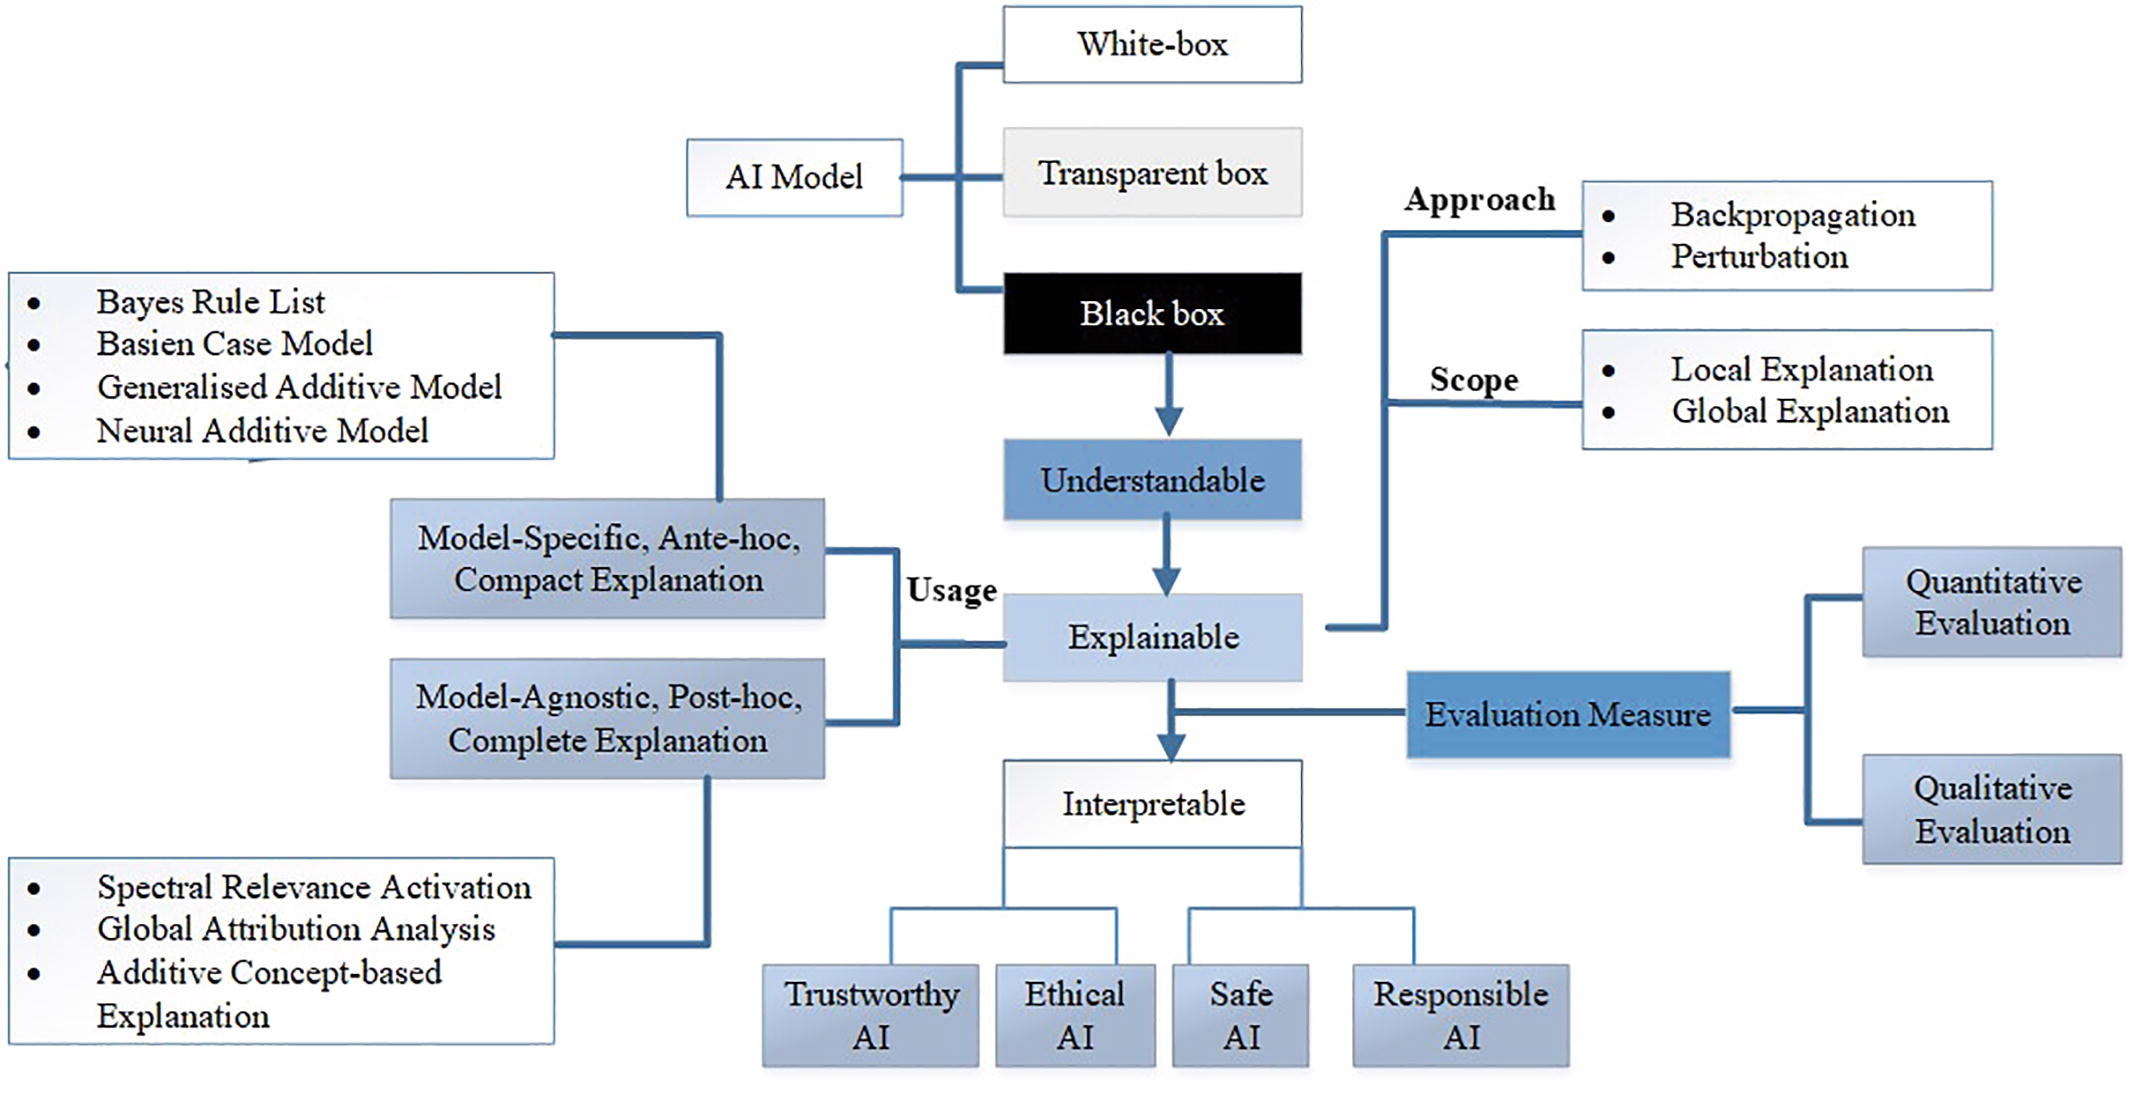
\includegraphics[width=1\textwidth]{images/CH02_algorithms_overview_Saleem.jpg}
    \caption{Explainability Overview, from \cite{SALEEM2022165}}
    \caption*{Overview of the concepts related to explainability algorithms.}
    \label{fig:Explainability_overview}
\end{figure}

The two most widely adapted local, model-agnostic, post-hoc methods are \textit{SHAP} (SHapley Additive exPlanations) \parencite{Lundberg2017} and \textit{LIME} (Local Interpretable Model-agnostic Explanations) \parencite{Ribeiro2016}.

\textbf{SHAP} is based upon the use of Shapley values used in coalitional game theory and aims to weight the importance of each feature to the result by game-theoretically distributing the value of the final prediction among all features being included \parencite{Molnar2023}.
The key features of SHAP are (based on \cite{Molnar2023})
\begin{itemize}
    \item \textbf{Additivity}: All feature contributions can be summed up in a linear way, benefitting understandability of the explanations.
    \item \textbf{Local Accuracy}: SHAP values are locally accurate, as predictions for a given input can be calculated as a result of the expected model output and the specific score for the local input.
    \item \textbf{Missingness}: As missingness in features is attributed zero values, missingness does not skew outcomes.
    \item \textbf{Consistency}: SHAP values do not change upon model change, but only when the actual feature contributions change.
\end{itemize}

\textbf{LIME} is based upon trying to approximate the model's decision boundary locally by perturbing the input data and observing the change in the model's output \parencite{Molnar2023}.

A way of globally assessing model explainability is the use of \textbf{(Global) Surrogate Models} (as opposed to e.g. the LIME algorithm, which can be considered a local surrogate model). 
These aim to make black-box algorithm decisions explainable by implementing white-box models to learn the decision criteria that the black-box model has established by being trained on the black-box predictions (compare e.g. \cite{Karim2023}).
Instead of making the predictions themselves explainable, these models aim to making the underlying decision criteria understandable \parencite{Molnar2023}.

\subsection{Explainability and Fairness}\label{subsec:Explainability_fairness}

%In order to conclude this literature review, this section will evaluate how the the concepts of fairness and explainability are related to each other, showing that the analysis of each adds separate value to this thesis.

Explainability and fairness within the field of Machine Learning do not inherently share the same scope. On the one hand, as an example, explainability is a rather objective concept, focusing on describing a model's inner workings neutrally. 
Comparing that to fairness it becomes apparent that the latter is a more subjective concept, as it is dependent on the context and man-made definitions, which are often rooted in certain (e.g.\ political) interpretations of fairness \parencite{Deepak2021}.
Yet, both concepts are somewhat dependent as assessing model fairness requires an understanding of the factors influencing a prediction \parencite{Zhou2022}.
Subsequently, approaches to connect both concepts have been proposed in academic literature. 
%Two different approaches are proposed by Deepak \parencite{Deepak2021}: 
%\begin{itemize}
%    \item \textbf{Interpretability for fairness (IFF)}: IFF is a framework intending to ensure that supposedly fair decisions made by AI are truly fair. The two steps in order to achieve that are \textit{clearly laying out the values supposed to adhered to} and \textit{explaining decisions made with regards to how they relate to those values}.
%    \item \textbf{Fairness and Interpretations (F\&I)}: F\&I is a multi-layered approach, which, in the first step, aims to satisfy both fairness and interpretability requirements based on given constraints. If both criteria in combination cannot satisfyingly be met, the user needs to be informed that the model is not sufficiently interpretable, but yet adheres to at least one of the two desired properties.
%\end{itemize}
However, these concepts are only stated on theoretical level without practical implications in this paper and are therefore not directly applicable for practitioners.


% Following Zhou's line of reasoning \parencite{Zhou2022}, other important approaches to merge the ideas of fairness and explainability in academic literature include:

% \textbf{Explanation as a way of guaranteeing fairness}: ... Papers!

% \textbf{Explanation as a way of shaping the perception of fairness}: ... Papers!

% \textbf{Perceived fairness of feature properties}: ... Papers!


Another promising approach to merge the concepts of fairness and explainability is the identification of root-causes for a certain model behavior by identifying \textit{influential subsets} within the underlying datasets as proposed by Pradhan \parencite{Pradhan2022}\footnote{For additional information on the proposed model see https://github.com/romilapradhan/gopher}.
By combining explainability criteria ('Why is a certain subgroup influential on the model's outcome?') with fairness criteria ('In how far can intervention in the training data regarding these subsets improve fairness?'), the authors manage to implement an efficient algorithm combining both concepts.

Just as it is the case for the aspect of fairness (as discussed in \textbf{chapter \ref{subsec:mortgage_lending_fairness}}), the field of mortgage lending has been specifically targeted by previous research on the aspect of explainability.
Maass et al. \parencite{Maass2022} contribute to the discussion by proposing the use of \textit{conceptual models} to capture the relationships in data, exemplarily using the HMDA 2020 dataset to predict mortgage approvals.
By using a total of 52 features clustered into different \textit{concepts} (i.e. abstracted groups of features), they determine the most important concepts relative to one another for the model's decision-making process.

In a comparative review of different explainability methods, Anderson evaluates the accuracy of explanations of different ML models on the 2019 HMDA dataset \parencite{Anderson2023}.
While all of the algorithms reviewed \textit{(most points lost, Shapley values, Shapley additive explanations, and the method of integrated gradients)} were able to provide explanations for the model's decisions, the accuracy of the explanations varied greatly between the different methods, with SHAP being the overall best-performing approach.

A very recent contribution to a research question from a similar field as this thesis has been made by Shiam et al. \parencite{Shiam2024}, who leverage explainable AI to assess the risk of credit default (as opposed to mortgage approval focused in this work), who leverage SHAP to explain predictions of a default classifier


%To-Do:
%Go through sources of Zhou and list important ones
%Mention specifically newly added analysis in this thesis
%Circle back to introduction: Why do both add value?

This thesis will add value to the discussion of fairness and explainability in Machine Learning by providing a novel approach to the analysis of both concepts in the field of mortgage lending: 
By using explainability algorithms and enrichment data, the analysis of fairness will be supported and iteratively adjusted with the aim of finding the optimal balance of both concepts.
%\chapter{Data}\label{ch:Data}

% Start with ‘what’ 
%  • What is the research question? And what kind of methods are suitable to answer it? 
%  • What kind of data you need to answer this? How was it collected? 
% Start with ‘why’ 
%  • Why is this valid methodology? 
% Don’t forget to cite all relevant papers  - probably on mortgage data or HMDA specifically

\section{HMDA Data}\label{sec:HMDA_Data}

% Follow structure from presentation Ana: From where, why, which steps etc. - probably add in appendix the code for the enrichment?

The underlying data for this analysis was obtained \textit{\href{https://ffiec.cfpb.gov/data-browser/data/2022?category=states}{via the HMDA Data Browser}}. \@
All data used are structured, tabular data that are publicly available. Privacy concerns are not relevant, as the data is anonymized.

XXX UPDATE! XXX

The data was filtered to only include entries from California, as it is the largest state in the US and thus provides a high amount of data. 
The time frame was set to 2022, as it is the most recent year available (!!!!!!!!!!). No filter was applied to the financial institutions, as the analysis is not focused on the institutions themselves. 
The data was further filtered to only include entries for single-family homes, as these are the most common type of homes and therefore provide the most data.

The raw dataset resulting from these filters contained $XXX$ entries and $XXX$ features, with a total sum of loan applications amounting to $XXX$ USD. The column types were $XXX$ of numeric, and $XXX$ of object dtype. $XXX$ columns contained missing values. \@
Due to the size of the dataset, a step-by-step description of the analysis and all cleaning steps taken is too extensive for this thesis. Therefore, this chapter will only outline the key assumptions incorporated, decisions made, and steps taken for data analysis and cleaning. For full detail, please refer to the corresponding notebook at XXX.

After the initial EDA, the first step was to \textit{drop} all features that are not relevant for the analysis in order to reduce dimensionality and improve the model learning process. \@ 
In this initial step, the amount of features was reduced from $XXX$ to $XXX$ with the following reasoning:
\begin{itemize}
    \item \textbf{activity\_year}: Does not provide value as the year is already pre-filtered
    \item \textbf{lei}: Does not matter as all financial institutions are used
    \item \textbf{derived\_msa-md}: Does not matter as county code is the geographical variable used in the analysis
    \item \textbf{state\_code}: Does not matter as the state is already pre-filtered
    \item \textbf{census\_tract}: Not relevant for the analysis
    \item \textbf{derived\_dwelling\_category} and \textbf{construction\_method}: Do not matter as the building category is already pre-filtered
    \item All information regarding \textbf{co-applicants} were dropped as the focus is on the main applicant
    \item All available \textbf{Reasons for Denial} were dropped as the focus is only on \textit{if} the loan was approved
    \item The dataset contains geographical information based on census tracts. As, however, the analysis of geographical features will be based on county level, the \textbf{census tract} is dropped.
\end{itemize}

The dataset contained both actual information on protected attributes (e.g.\ \mbox{applicant\_ethnicity-1} to \mbox{applicant\_ethniciy-5}) and derived information that aggregate the former into one overarching category (e.g.\ \mbox{derived\_ethnicity}). 
As this analysis focuses on fairness concerns, where such protected attributes play an important role, the derived information was dropped in favor of the actual information in order to achieve a higher granularity of this important type of data.  
However, as only few applicants have made use of all the fields (for example, only 0.07\% of applicants have reported more than two ethnicities), the amount of features was reduced by only including the top two selections for each protected attribute. 
This was done in order to avoid a high amount of missing values in the dataset as well as to strike a balance between the amount of features (and therefore model performance) and the granularity of the data.

Several columns contained a very high amount of missing values XXX DETAIL OF FINAL DATA HERE? XXX. In order to assess how to proceed with them, the missingness was analyzed closer. While the amount of available features would have allowed for the \textit{dropping} of predominantly missing feature columns, this might have introduced bias or impacted variable distributions if the missingness was not completely at random (MCAR).
Therefore, missingness was analyzed numerically and visually (see \textbf{Figure \ref{fig:CH03_OLD!_Missingno_Completeness}} for how the missingno package was utilized to scan for patterns in the missingness), leading to the following procedure decision for the features with the highest amounts of missing values:

\begin{figure}[h]
    \centering
    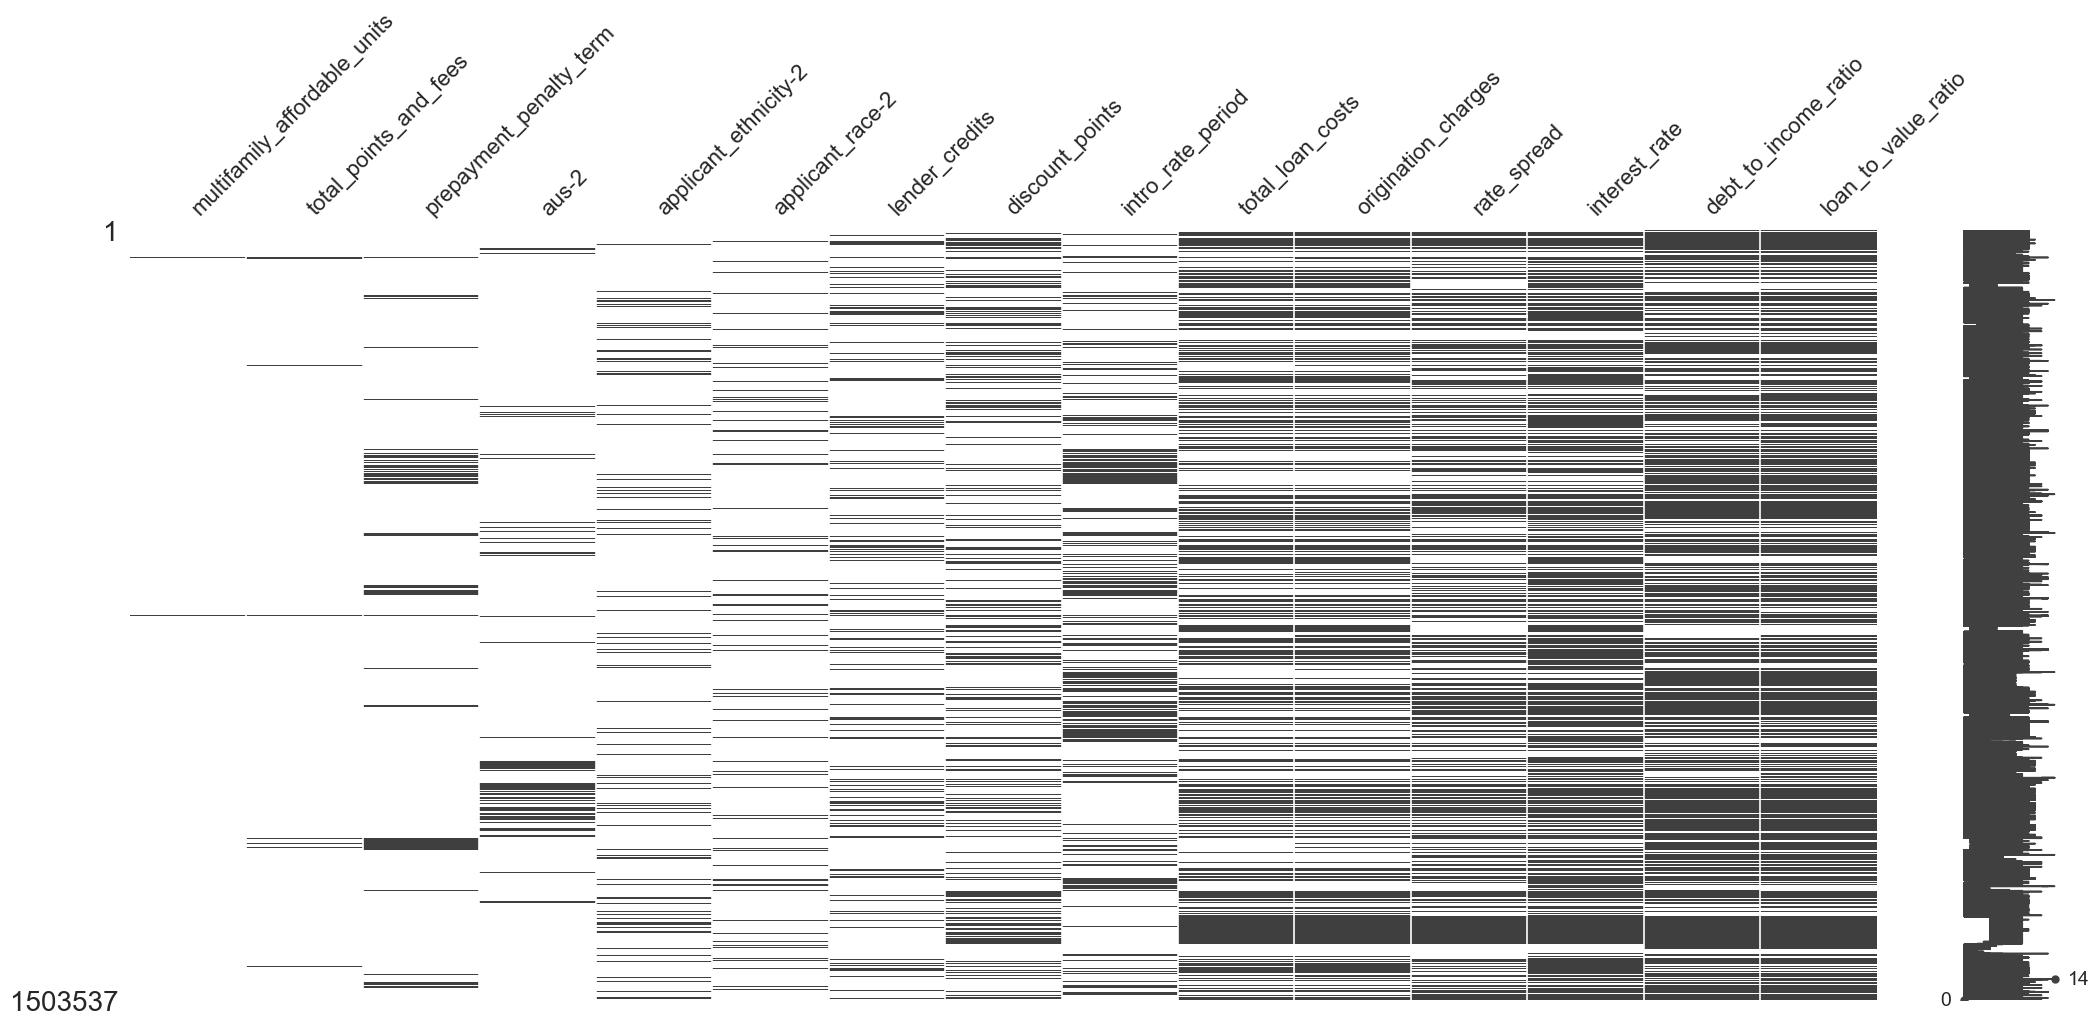
\includegraphics[width=0.85\textwidth]{images/CH03_OLD!_Missingno_Completeness.png}
    \caption{Visual Inspection of Missingness in the missingno package}
    \label{fig:CH03_OLD!_Missingno_Completeness}
\end{figure}

\begin{itemize}
    \item \textbf{multifamily\_affordable\_units}: This column seems to be erroneous, as it contains only one unique value ("Exempt"), whereas it is supposed to contain percentages according to the documentation. It is therefore dropped.
    \item \textbf{total\_points\_and\_fees}, \textbf{prepayment\_penalty\_term}, \textbf{lender\_credits}, \textbf{discount\_points}, and \textbf{intro\_rate\_period}: These might have been interesting to include in the analysis. However, the sheer amount of missingness (which seems to be MCAR from visual inspection) makes them unsuitable for the analysis. They are therefore dropped.
    \item \textbf{aus-2}: This column refers to a second underwriting system for the loan. As the vast majority of loans only have one underwriting system and, opposed to the second variables for the protected attributes, information on aus-2 does not add value to the analysis, this column is dropped.
    \item \textbf{applicant\_ethnicity-2} and \textbf{applicant\_race-2}: As discussed above, these are part of the highly important protected attributes. Even though the amount of missing values is high and imputation is not suitable here for logical reasons, these columns will be kept including their missing values in order to not lose the granularity of the data.
    \item \textbf{total\_loan\_costs} and \textbf{origination\_charges} are (expectably) heavily correlated. In order to benefit the analysis, one of them (origination\_charges) is dropped, while the other is kept for further analysis on how to handle the missing values.
    \item \textbf{rate\_spread} and \textbf{interest\_rate} are highly important variables for the analysis. However, the amount of missing values is high. As the missingness seems to be MAR from visual inspection, imputation of the missing values will be tried.
    \item \textbf{debt\_to\_income\_ratio} and \textbf{loan\_to\_value\_ratio} are highly correlated. In order to benefit the analysis, one of them (debt\_to\_income\_ratio) is dropped, while the other is kept for further analysis on how to handle the missing values.
\end{itemize}

% Exempt: Reasoning for imputation, procedure, graphs - not strictly logical but ok for modelling reasons and not many values
% Remove initial outliers to check distribution for initial imputation - comment on distributions
% Data Types: Except inferral and categorization - note: Some of the columns need further recasting (e.g. float to int / vice versa or numerical to categorical). At this stage however, the data is prepared for the next steps.
% Missingness: Four different strategies based on type of missingness (go into detail imputation and maybe use graph or two)
% Step to second workbook and comment where to find
% New category casting for analysis - describe examples like str for cc and cat for categorical
% Further refinement of protected attributes (dropping of useless values, renaming of categories, etc.)
% Basic EDA of distributions for protected attributes


\section{Enrichment Data}\label{sec:Enrichment_Data}

% Follow structure from presentation Ana: From where, why, which steps etc. - probably add in appendix the code for the enrichment?

The enrichment data was obtained from the \textit{\href{https://www.ers.usda.gov/data-products/county-level-data-sets/}{USDA ERS page}}. All data used are structured, tabular data that are publicly available. Privacy concerns are not relevant, as the data is anonymized and aggregated. All available reports were downloaded, specifically the following datasets:

\begin{itemize}
    \item \textbf{Poverty} (2021 latest)
    \item \textbf{Population} (2022 latest)
    \item \textbf{Unemployment, and Median Household Income} (annual average 2022 unemployment and 2021 median income latest)
    \item \textbf{Education} (2017–21, 5-year average latest).
\end{itemize}

In order to clean and reshape the data in a easily analyzable format, the following steps were taken\footnote{For all detail, see the corresponding cleaning notebook at !!! XXX !!!}:
All datasets were \textit{filtered} to only contain CA county-level data, not the aggregated values for the full state of California and, in case multiple years of analysis were available, to only include the newest datapoints. 
Where there were more features available than would be useful for the analysis, the datasets were \textit{reduced} to only include the most relevant features, being:

\begin{itemize}
    \item \textbf{Poverty:} Only the percentage of the population living in poverty (PCTPOVALL\_2021) was included
    \item \textbf{Population:} Only the total population (POP\_ESTIMATE\_2022) was included
    \item \textbf{Unemployment, and Median Household Income:} The unemployment rate (Unemployment\_rate\_2022) and the median household income (Median\_Household\_Income\_2021) were included
    \item \textbf{Education:} All relative values, i.e.\ percentages of adults with their corresponding highest degrees were included.
\end{itemize}

All datasets were \textit{pivoted} in order to use the attributes as feature names and \textit{indexed} by the FIPS code and the name of the respective county. After basic \textit{checks for completeness}, the feature columns were \textit{renamed} for clarity. Finally, all datasets were \textit{merged} into a single dataframe, which was then \textit{exported} as a pickle file for further use in the analysis.

% Reasoning!

The cleaned data are \textit{complete} in a way that there are values available for all features and for all of the 58 counties. Basic summary statistics can be found in \textbf{Table \ref{tab:enrichment_summary}}. Expectedly, there is a high correlation between some of the features, see \textbf{Figure \ref{fig:CH03_Enrichment_Correlation}}.

\begin{table}[h]
    \centering
    \begin{tabularx}{\textwidth}{llllll}
    \hline
     & \textbf{Count} & \textbf{Mean} & \textbf{Std} & \textbf{Min} & \textbf{Max} \\
    \hline
    College Degree (Perc.) & 58.00 & 33.19 & 5.77 & 17.89 & 44.23 \\
    \hline
    Bachelor Degree or Higher (Perc.) & 58.00 & 28.55 & 12.27 & 11.77 & 60.15 \\
    \hline
    High School Degree (Perc.) & 58.00 & 23.77 & 5.84 & 10.17 & 38.42 \\
    \hline
    Less than High School Degree (Perc.) & 58.00 & 14.49 & 7.02 & 4.87 & 29.65 \\
    \hline
    Population (thousands) & 58.00 & 672.92 & 1,428.89 & 1.19 & 9,721.14 \\
    \hline
    Poverty Rate (Perc.) & 58.00 & 13.63 & 3.96 & 6.60 & 21.90 \\
    \hline
    Median Household Income (thousands) & 58.00 & 75.30 & 21.89 & 45.51 & 141.16 \\
    \hline
    Unemployment Rate (Perc.) & 58.00 & 4.84 & 2.07 & 2.40 & 14.70 \\
    \hline
    \end{tabularx}
    \caption{Summary Statistics of the Enrichment Data}
    \label{tab:enrichment_summary}
\end{table}

\begin{figure}[h]
    \centering
    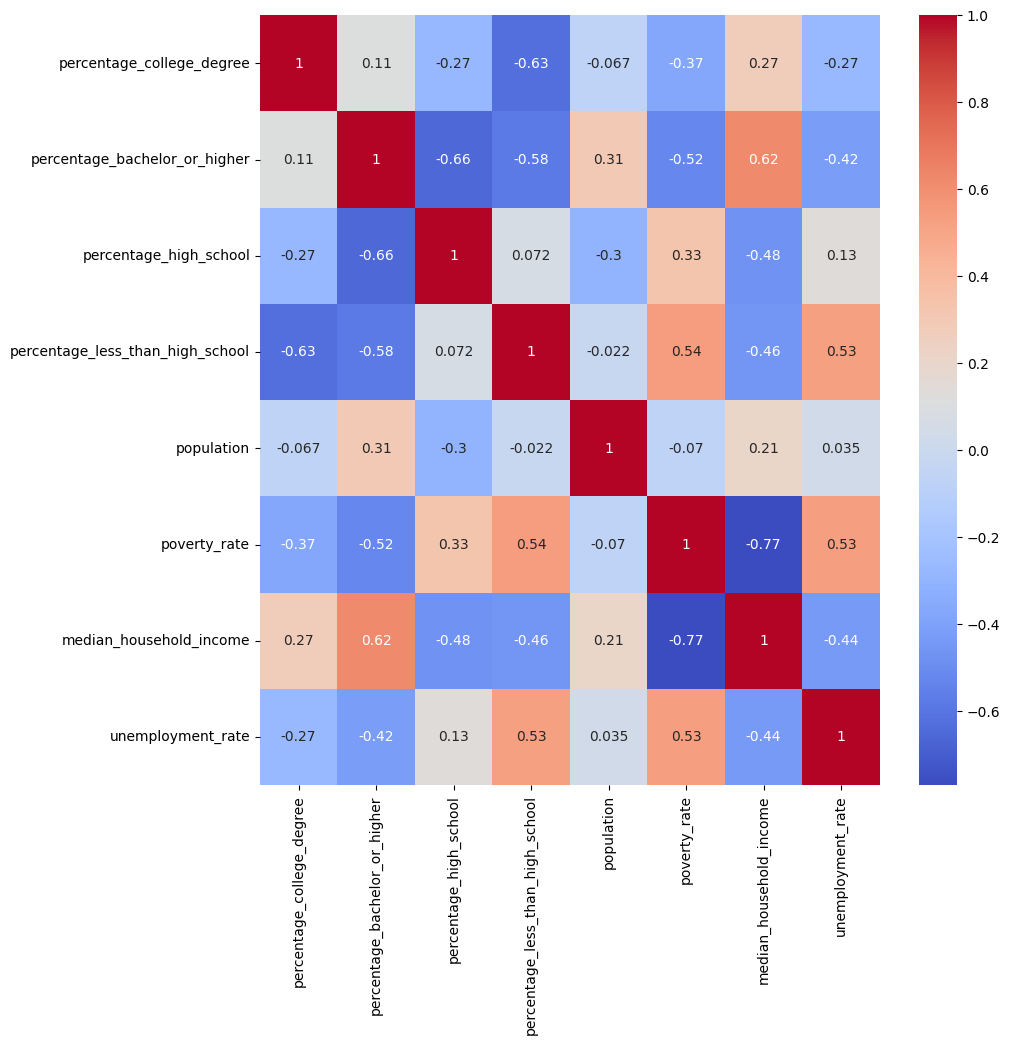
\includegraphics[width=0.85\textwidth]{images/CH03_Enrichment_Correlation.png}
    \caption{Correlation Between the Enrichment Features}
    \label{fig:CH03_Enrichment_Correlation}
\end{figure}
\chapter{Data and Methodology}\label{ch:Data_and_Methodology}



\section{Data}\label{sec:Data}



\subsection{HMDA Data}\label{subsec:HMDA_Data}

% Follow structure from presentation Ana: From where, why, which steps etc. - probably add in appendix the code for the enrichment?

The underlying data for this analysis was obtained \textit{\href{https://ffiec.cfpb.gov/data-browser/data/2022?category=states}{via the HMDA Data Browser}}. \@

XXX UPDATE! XXX

The data was filtered to only include entries from California, as it is the largest state in the US and thus provides a high amount of data. 
The time frame was set to 2022, as it is the most recent year available (!!!!!!!!!!). No filter was applied to the financial institutions, as the analysis is not focused on the institutions themselves. 
The data was further filtered to only include entries for single-family homes, as these are the most common type of homes and therefore provide the most data.

The raw dataset resulting from these filters contains $XXX$ entries and $XXX$ features, with a total sum of loan applications amounting to $XXX$ USD.

\subsection{Enrichment Data}\label{subsec:Enrichment_Data}

% Follow structure from presentation Ana: From where, why, which steps etc. - probably add in appendix the code for the enrichment?

The enrichment data was obtained from the \textit{\href{https://www.ers.usda.gov/data-products/county-level-data-sets/}{USDA ERS page}}. All available reports were downloaded, specifically the following datasets:

\begin{itemize}
    \item \textbf{Poverty} (2021 latest)
    \item \textbf{Population} (2022 latest)
    \item \textbf{Unemployment, and Median Household Income} (annual average 2022 unemployment and 2021 median income latest)
    \item \textbf{Education} (2017–21, 5-year average latest).
\end{itemize}

In order to clean and reshape the data in a easily analyzable format, the following steps were taken\footnote{For all detail, see the corresponding cleaning notebook at !!! XXX !!!}:
All datasets were \textit{filtered} to only contain CA county-level data, not the aggregated values for the full state of California and, in case multiple years of analysis were available, to only include the newest datapoints. 
Where there were more features available than would be useful for the analysis, the datasets were \textit{reduced} to only include the most relevant features, being:

\begin{itemize}
    \item \textbf{Poverty:} Only the percentage of the population living in poverty (PCTPOVALL\_2021) was included
    \item \textbf{Population:} Only the total population (POP\_ESTIMATE\_2022) was included
    \item \textbf{Unemployment, and Median Household Income:} The unemployment rate (Unemployment\_rate\_2022) and the median household income (Median\_Household\_Income\_2021) were included
    \item \textbf{Education:} All relative values, i.e.\ percentages of adults with their corresponding highest degrees were included.
\end{itemize}

All datasets were \textit{pivoted} in order to use the attributes as feature names and \textit{indexed} by the FIPS code and the name of the respective county. After basic \textit{checks for completeness}, the feature columns were \textit{renamed} for clarity. Finally, all datasets were \textit{merged} into a single dataframe, which was then \textit{exported} as a pickle file for further use in the analysis.

% Reasoning!

The cleaned data are \textit{complete} in a way that there are values available for all features and for all of the 58 counties. Basic summary statistics can be found in \textbf{Table \ref{tab:enrichment_summary}}. Expectedly, there is a high correlation between some of the features, see \textbf{Figure \ref{fig:CH03_Enrichment_Correlation}}.

\begin{table}[h]
    \centering
    \begin{tabularx}{\textwidth}{llllll}
    \hline
     & \textbf{Count} & \textbf{Mean} & \textbf{Std} & \textbf{Min} & \textbf{Max} \\
    \hline
    College Degree (Perc.) & 58.00 & 33.19 & 5.77 & 17.89 & 44.23 \\
    \hline
    Bachelor Degree or Higher (Perc.) & 58.00 & 28.55 & 12.27 & 11.77 & 60.15 \\
    \hline
    High School Degree (Perc.) & 58.00 & 23.77 & 5.84 & 10.17 & 38.42 \\
    \hline
    Less than High School Degree (Perc.) & 58.00 & 14.49 & 7.02 & 4.87 & 29.65 \\
    \hline
    Population (thousands) & 58.00 & 672.92 & 1,428.89 & 1.19 & 9,721.14 \\
    \hline
    Poverty Rate (Perc.) & 58.00 & 13.63 & 3.96 & 6.60 & 21.90 \\
    \hline
    Median Household Income (thousands) & 58.00 & 75.30 & 21.89 & 45.51 & 141.16 \\
    \hline
    Unemployment Rate (Perc.) & 58.00 & 4.84 & 2.07 & 2.40 & 14.70 \\
    \hline
    \end{tabularx}
    \caption{Summary Statistics of the Enrichment Data}
    \label{tab:enrichment_summary}
\end{table}

\begin{figure}[h]
    \centering
    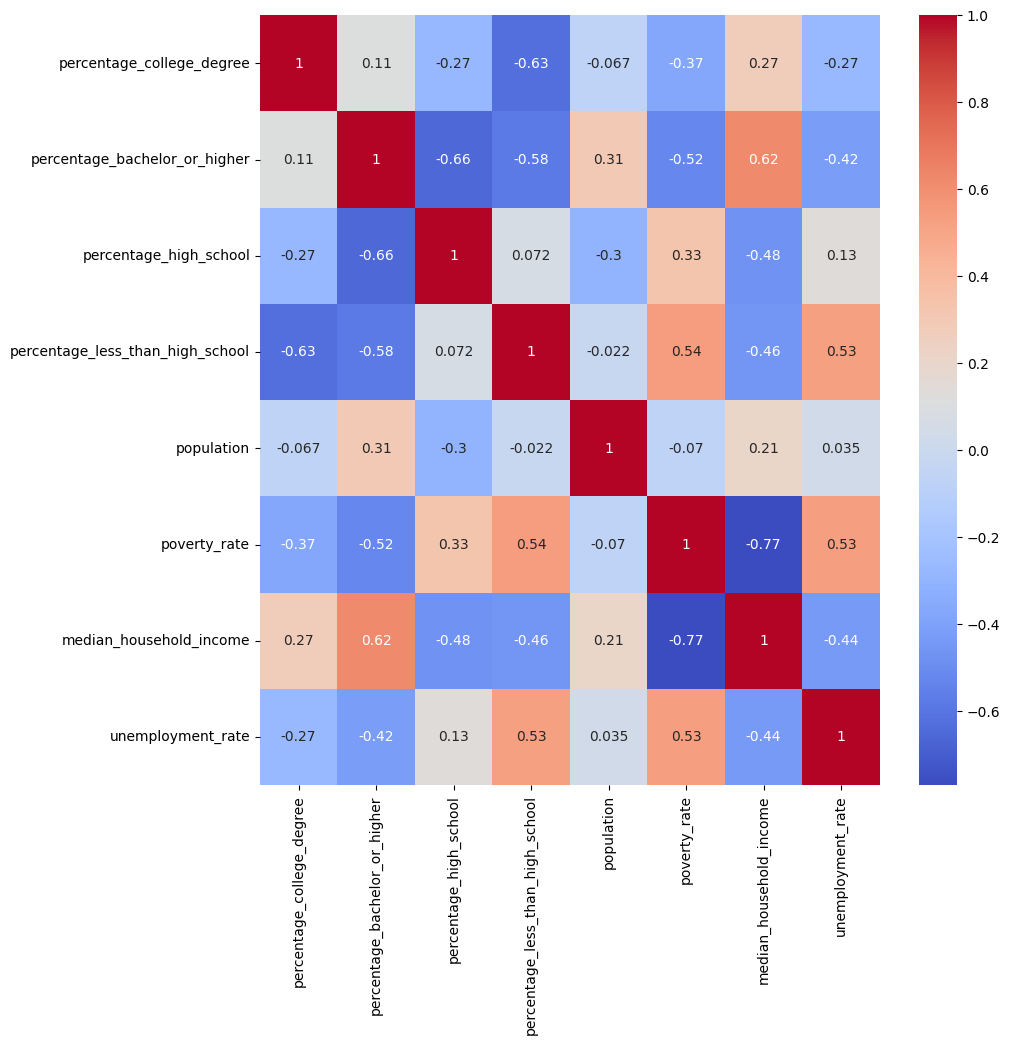
\includegraphics[width=0.7\textwidth]{images/CH03_Enrichment_Correlation.png}
    \caption{Correlation Between the Enrichment Features}
    \label{fig:CH03_Enrichment_Correlation}
\end{figure}

\section{Methodology}\label{sec:Methodology}

% appendix

\printbibliography

\end{document}